\documentclass[11p]{article}
% Packages
\usepackage{amsmath}
\usepackage{graphicx}
\usepackage[swedish]{babel}
\usepackage[
    backend=biber,
    style=authoryear-ibid,
    sorting=ynt
]{biblatex}
\usepackage[utf8]{inputenc}
\usepackage[T1]{fontenc}
%Källor
\addbibresource{mall.bib}
\graphicspath{ {./images/} }

\title{PMmall \\ \small Fysik 1}
\author{Endo Axelsson }
\date{\today}


\begin{document}

    \begin{titlepage}
        \begin{center}
            \vspace*{1cm}

            \Huge
            \textbf{Title}

            \vspace{0.5cm}
            \LARGE
            Subtitle

            \vspace{1.5cm}

            \textbf{Author Name}

            \vfill

            Ett PM om energiförsörjning \\
            Fysik 1

            \vspace{0.8cm}

            
\includegraphics[width=0.4\textwidth]{../images/NTI Gymnasiet_Symbol_print_svart.png}

            \Large
            Teknikprogrammet\\
            NTI Gymnasiet\\
            Umeå\\
            \today

        \end{center}
    \end{titlepage}
% Om arbetet är långt har det en innehållsförteckning, annars kan den utelämnas
    \tableofcontents
    \newpage
    \section{Disposition hos ett PM}
    Ett PM har den mest informella strukturen av de vetenskapliga texterna. Det är egentligen bara en sammanställning av kunskap men för att den ska bli lite lättare att ta sig an brukar det finnas en inledning där syfte och frågeställningar redovisas och en avslutning där du kan dra slutsatser. Rubrikerna kan döpas valfritt, speciellt de som finns i huvuddelen av texten beror på vad den handlar om. Se nedan för ett exempel.

    \section{Inledning}
    Vi behöver en ny och mer miljövänlig energikälla för jordens hälsa långsiktigt.
    En energikälla som inte är  beroende av olja och brännbara fossiler.
    Detta är ett relevant ämne som diskuterass runtom hela världen.
    Vilken källa är bäst och hur mycket av det finns det?
    Dem naturliga energikällorna är temat som pratas mycket om och vindkraft är en av dem.
    Men som allt annat så har allt positivt också något negativt och vindkraft är inte ett undantag.
    Så det finns det såklart frågor runtom vindkraften också.
    \subsection{frågeställningar}
    \begin{enumerate}
        \item Vindkraft, så fungerar det
        \item Globala och lokala miljöpåverkan av vindkraft
        \item Vindkraftens påverkan på områden och ekonomi
        \item Vindkraft, land eller vatten?
    \end{enumerate}

    \section{Resultat}

    \subsection{Vindkraft, så fungerar det}

    Vindkraftens koncept på hur den fungerar är rätt så simpelt.
    Som namnet utger så kommer energin från vinden

    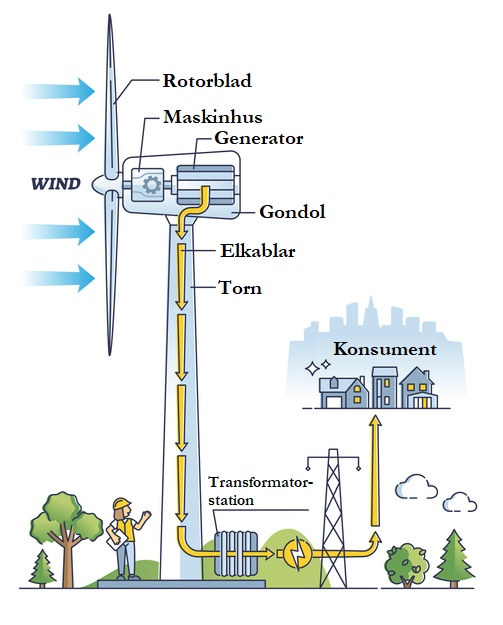
\includegraphics[width=0.6\textwidth]{../images/vindhur.jpg}
    \caption{funktionen i princip. Källa: Ugglasno.se}

    \subsection{Globala och lokala miljöpåverkan av vindkraft}
    \subsection{Vindkraftens påverkan på områden och ekonomi}
    \subsection{Vindkraft, land eller vatten?}

    \includegraphics[width=1\textwidth]{../images/vindterräng.jpg}

    \subsection{}

    \section{Slutsatser}
    Här kan du dra slutsatser eller sammanfatta ditt resultat

% Mer saker som du kan ha nytta av.

    \section{Referenser}
    Referenser i text kan skrivas på två sätt: Enligt \textcite{Jens} kan man använde två typer av referenser, inbäddade i texten eller efter ett fakta \parencite{Fraenkel}. Ett till test för att se hur det ser ut \parencite[sid 55]{fermi}.

    \section{Annat som kan vara bra att veta}
    Om du vill ha kodstil och få med alla tecken kan du använda verbatim. då kan du skriva \verb|abcd!"#| utan problem...

    Citat skrivs mellan de konstiga symbolerna \verb|``| och \verb|''| för att de ska se bra ut ``se bra ut!''.
    \subsection{En underrubrik}
    \subsubsection{En underunderrubrik}
    \subsection{Ekvationer}
    Det är lätt att skriva matematik i \LaTeX

    \begin{equation}
        F = G \frac{M m}{r^2}
        \label{grav}
    \end{equation}

    Ekvation (\ref{grav}) känner ni igen...

    \subsection{figurer}
    Bilder placeras enklast på detta sätt. placeringen bestämmer \LaTeX och vi kan bara föreslå (h)är, (t)opp eller (b)otten. Ett utropstecken före tvingar lite mer men inte absolut. I bild \ref{varg} visas en varg
    \begin{figure}[!h]
        \includegraphics[width=0.8\textwidth]{../images/accelerationTime.png}
        \caption{Acceleration-tid diagram. Källa: Impuls Fysik 1}
        \label{varg}
    \end{figure}
    \printbibliography

\end{document}
